\section{Graphs of Tables of Critical Frequencies} \label{Graphs_Tables}

\subsection{Implicational quantifiers}
Let us return to the end of section \ref{Graphs}, where problem of correlation between the \emph{founded implication}, \emph{lower} and \emph{upper critical implication}. Previous section showed, that these quantifiers are \emph{implicational} and one can create \emph{tables of maximal b's} for the quantifiers. This fact means a reduction of one to two dimensions (variable $p$ and $b$ of critical implications) and possibility of comparing the quantifiers. Figure \ref{fig:Implicational} displays graphs of maximal b's for $p=0.8$, $\alpha=0.05$ and for $a=0\dots1000$.

\begin{figure}[ht]
\centering
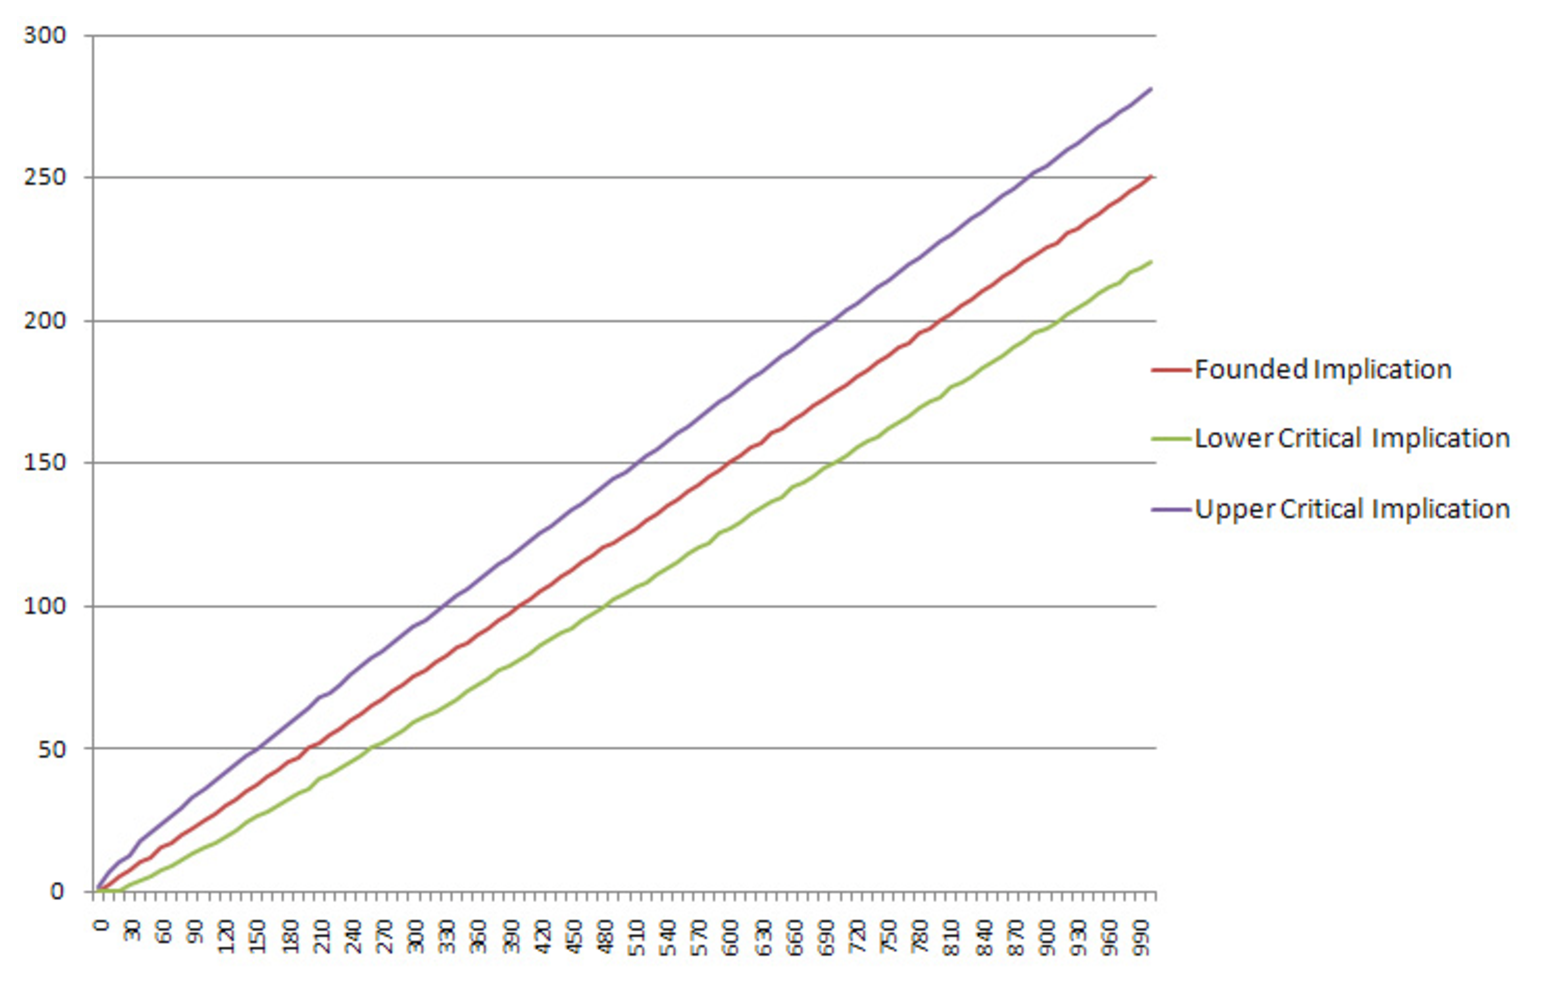
\includegraphics[width=115mm]{Implicational.eps}
%\mbox{\resizebox{125mm}{!}{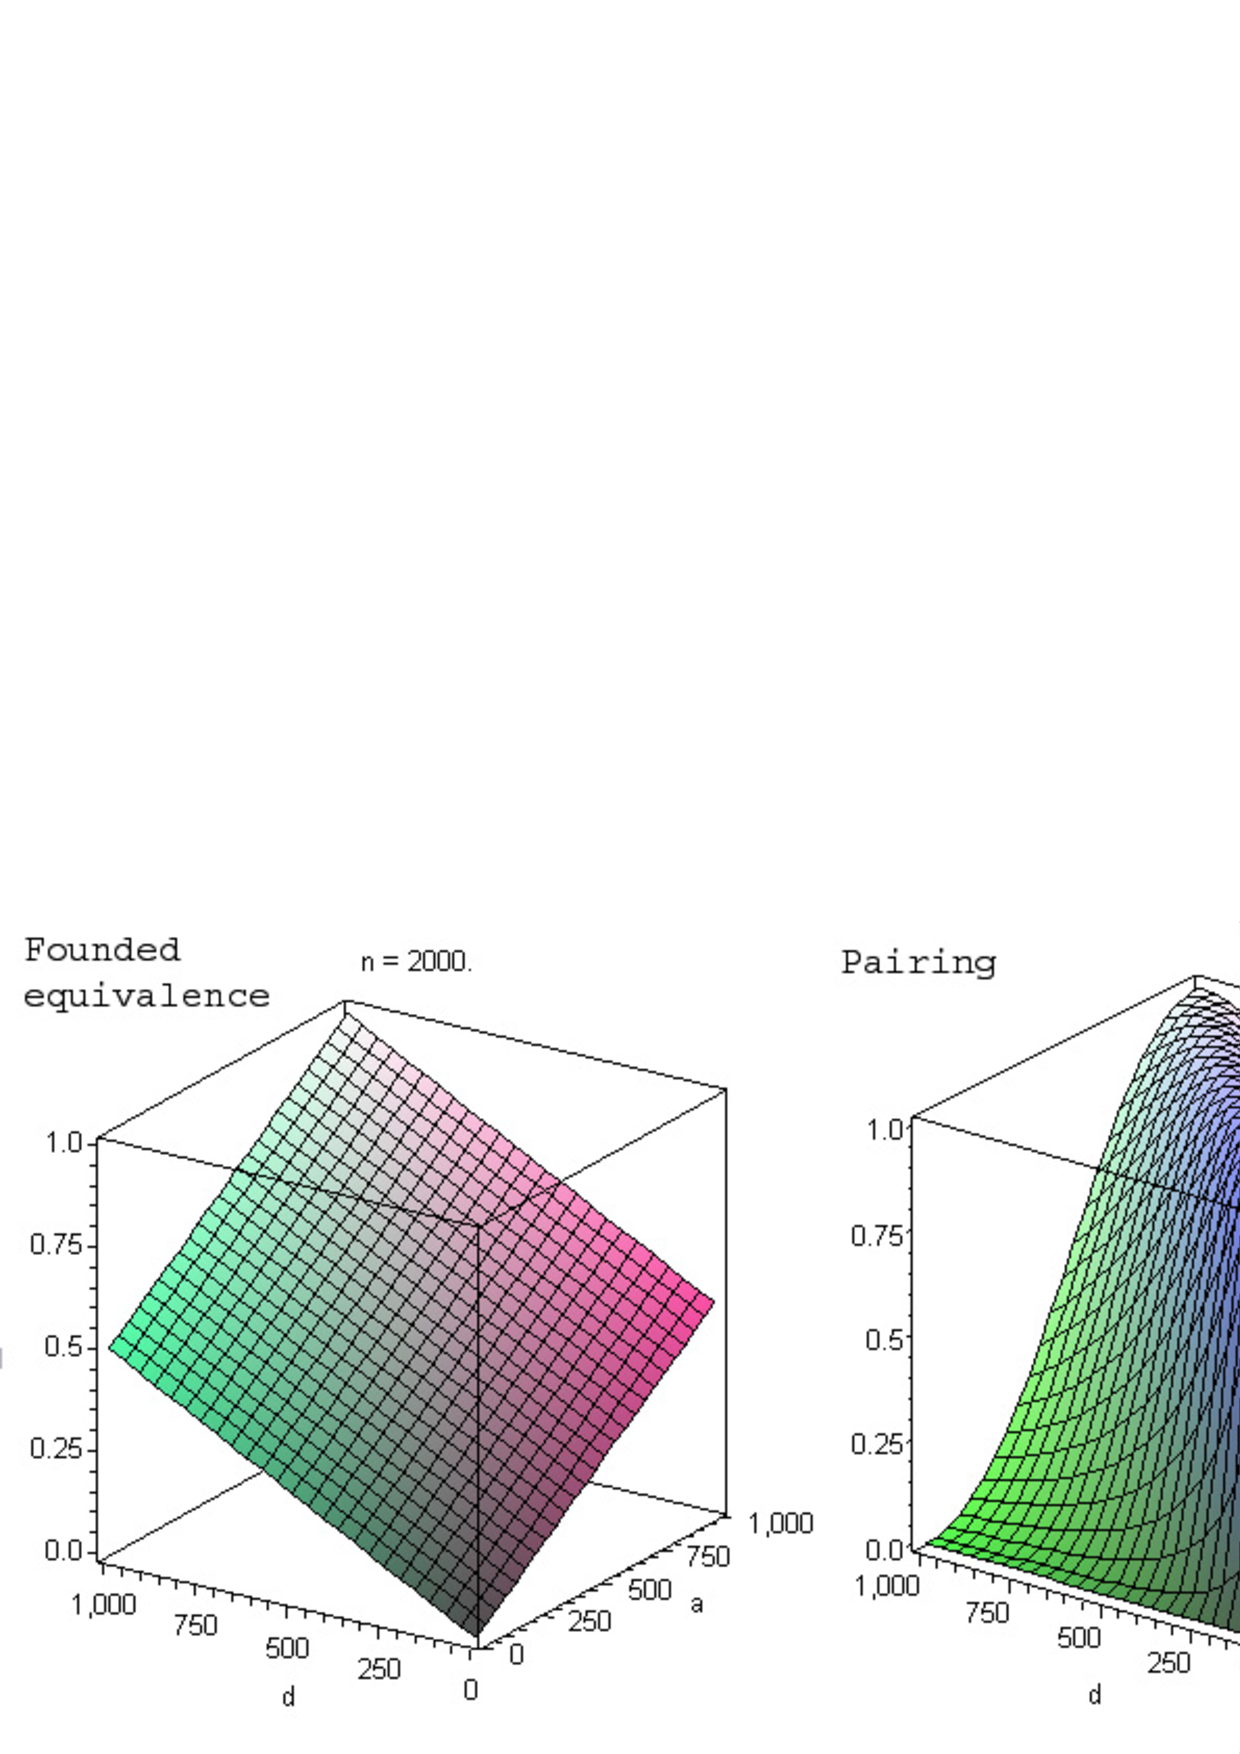
\includegraphics{FE-Pairing.png}}}
\caption{Tables of maximal b's for implicational quantifiers}
\label{fig:Implicational}
\end{figure}

The graph shows, that we cannot use (in the examined range of $a$) computationally simple \emph{founded implication} instead of statistically sound but computationally demanding \emph{lower} and \emph{upper critical implications}. This is an important result that could not be obtained without construction of \emph{tables of maximal b's}.

We can think of \emph{tables of maximal b} as another definition of the quantifier. It is function from $a$ to $b$. For \emph{founded implication} we know exact definition of the function. It is 
%
%
%$f(a) = \frac{a(1-p)}{p}$ 
%
%VERSE RAUCH:
$ Tb_{\Rightarrow_{p}} = \left\lceil \frac{a(1-p)}{p} + 1 \right\rceil$
%
and can be obtained by basic arithmetic operations, $ \left\lceil x \right\rceil$ means upper integer part of $x$. 
To our best knowledge, arithmetic extraction of the function for critical implications is impossible. For construction of the table, we programmed iterations over $a$ and $b$ and checked, when the evaluation function stops being valid. This is computationally demanding because of the factorials in binomial coefficient and cannot be done effectively for very high numbers. Thus we can only guess the behavior of these functions close to infinite values. 

To get a better idea about the functions, we examined their slopes (or first derivatives). It is constant for \emph{founded implication} and equals the $\frac{1-p}{p}$. Slopes of the critical implication in chosen points ($a$ values) are shown in table \ref{tab:slopes}.

\begin{table}[ht]
	\centering
		\begin{tabular}{|p{4cm}|p{1cm}|p{1cm}|p{1cm}|p{1cm}|p{1cm}|p{1cm}|p{1cm}|}
			\hline
			&\textbf{10}&\textbf{100}&\textbf{300}&\textbf{500}&\textbf{700}&\textbf{900}&\textbf{1000}\\
			\hline
			\textbf{Lower Critical Impl.}&0.1&0.16&0.2&0.21&0.215&0.22&0.22\\
			\hline
			\textbf{Upper Critical Impl.}&0.7&0.36&0.306&0.294&0.285&0.282&0.281\\
			\hline
		\end{tabular}
	\caption{Slopes of critical frequencies}
	\label{tab:slopes}
\end{table}

The table reveals interesting facts. Note, that the difference between slopes of critical implications and slope of \emph{founded implication} remains the same. This means that the critical implications maximal b's tables are symmetric with respect to the \emph{founded implication} maximal b table. 

Our working hypothesis is, that 
%$$\lim_{a\rightarrow\infty} \frac{Tb_{\Rightarrow^{!}_{p, \alpha}}}{da} = \lim_{a\rightarrow\infty} %\frac{Tb_{\Rightarrow^{?}_{p, \alpha}}}{da} = \lim_{a\rightarrow\infty} \frac{dTb_{\Rightarrow_{p}}}{da} = %\frac{dTb_{\Rightarrow_{p}}}{da} = \frac{1-p}{p}$$ 
%
%
%VERSE RAUCH
%
$$\lim_{a\rightarrow\infty} \frac{Tb_{\Rightarrow^{!}_{p, \alpha}}(a)}{a} = \lim_{a\rightarrow\infty} \frac{Tb_{\Rightarrow^{?}_{p, \alpha}}(a)}{a} = \lim_{a\rightarrow\infty} \frac{Tb_{\Rightarrow_{p}}(a)}{a} = %\frac{dTb_{\Rightarrow_{p}}}{da} = 
\frac{1-p}{p} \mbox{ .}$$ 

However we are currently unable to prove it. If our hypothesis is correct, for all natural $a$, 
$Tb_{\Rightarrow^{!}_{p, \alpha}}(a) < Tb_{\Rightarrow_{p}}(a) < Tb_{\Rightarrow^{?}_{p, \alpha}}(a)$,
thus one can never replace critical implications with \emph{founded implication}.

\subsection{Quantifiers with F-property}
For quantifiers with the F property, we constructed \emph{tables of minimal $|b-c|$'s}. The construction algorithm worked in two steps: the first step was to find $(a,b,c,d)$ quadruples that satisfied the quantifier. The second step was to find for given $a$ and $d$ the maximal $|b-c|$ for the quadruples. This way a matrix indexed with $a$ and $d$ containing minimal still valid $|b-c|$ was obtained. The matrix subsequently transformed to a graph. 

The most interesting result is the comparison of the \emph{simple deviation} and \emph{Fisher's} quantifiers. The results are displayed in figure \ref{fig:FProperty}, where graphs of tables of critical frequencies for $n=10$ and $n=1000$ are shown, $\alpha=0.05$ and $\delta=0$.

\begin{figure}[ht]
\centering
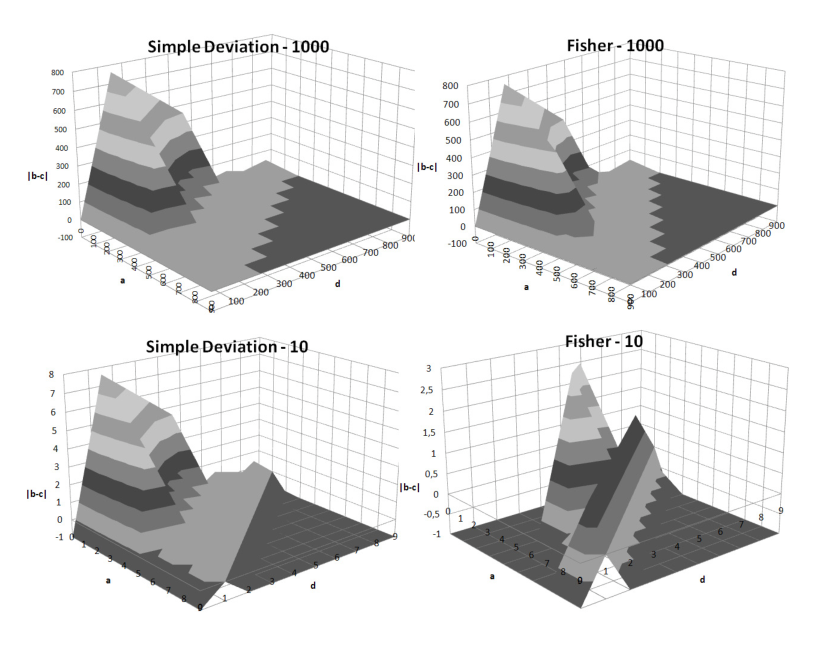
\includegraphics[width=115mm]{SDFisher.eps}
%\mbox{\resizebox{125mm}{!}{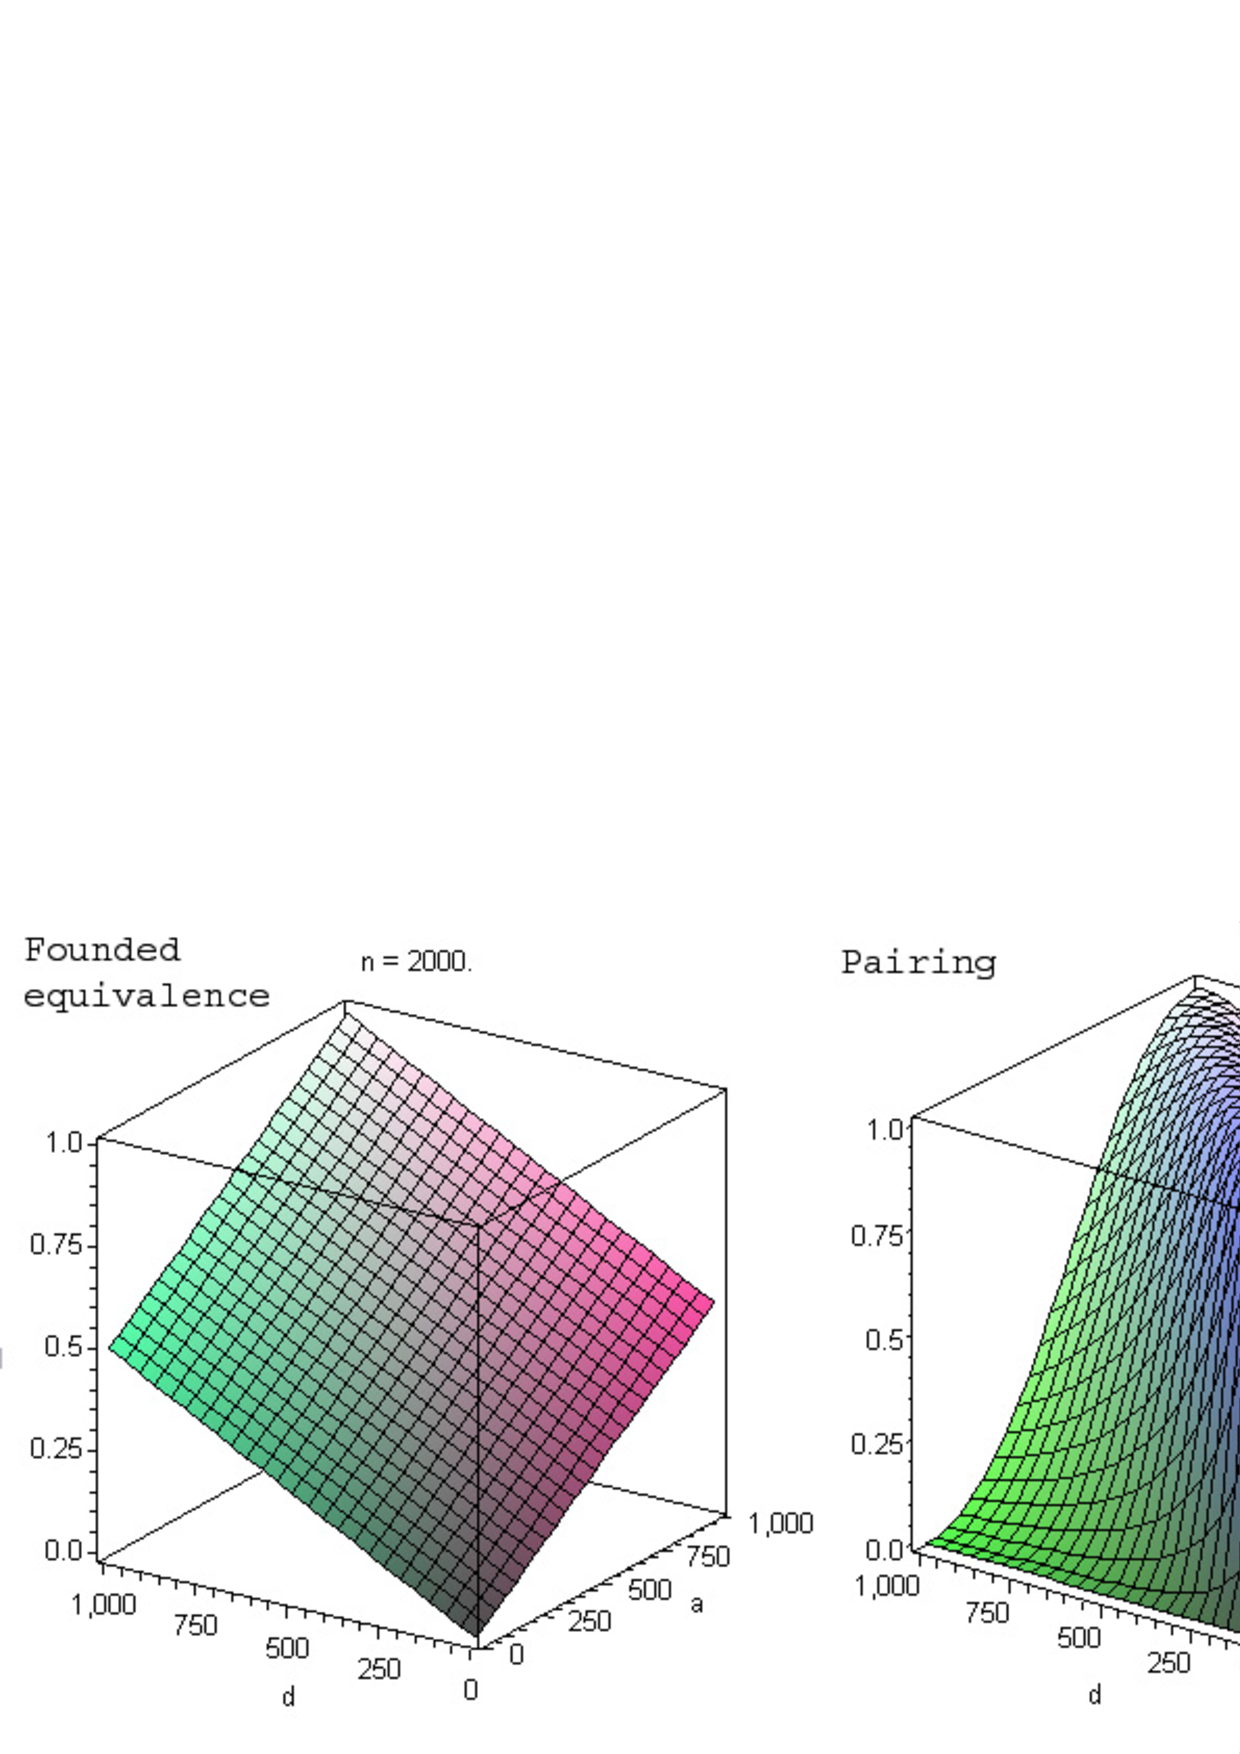
\includegraphics{FE-Pairing.png}}}
\caption{Tables of minimal $|b-c|$ for Fisher and Simple Deviation quantifiers}
\label{fig:FProperty}
\end{figure}

For the larger table, the Fisher's graph is approximately the same as graph of \emph{simple deviation}. We did not compute values of the graph in all the possible points, we chose 100 representative points instead. Therefore the graphs only estimate real \emph{tables of minimal $|b-c|$}. Yet the estimates are the same for both quantifiers.

For the smaller table, the \emph{simple deviation} graph remains in the shape of the graph from the larger table. The \emph{Fisher's} quantifier graph does retain the shape, the quantifier is valid only in a small area near the center of the graph. The resemblance of the graphs remains an open question. 

\begin{figure}[h]
\centering
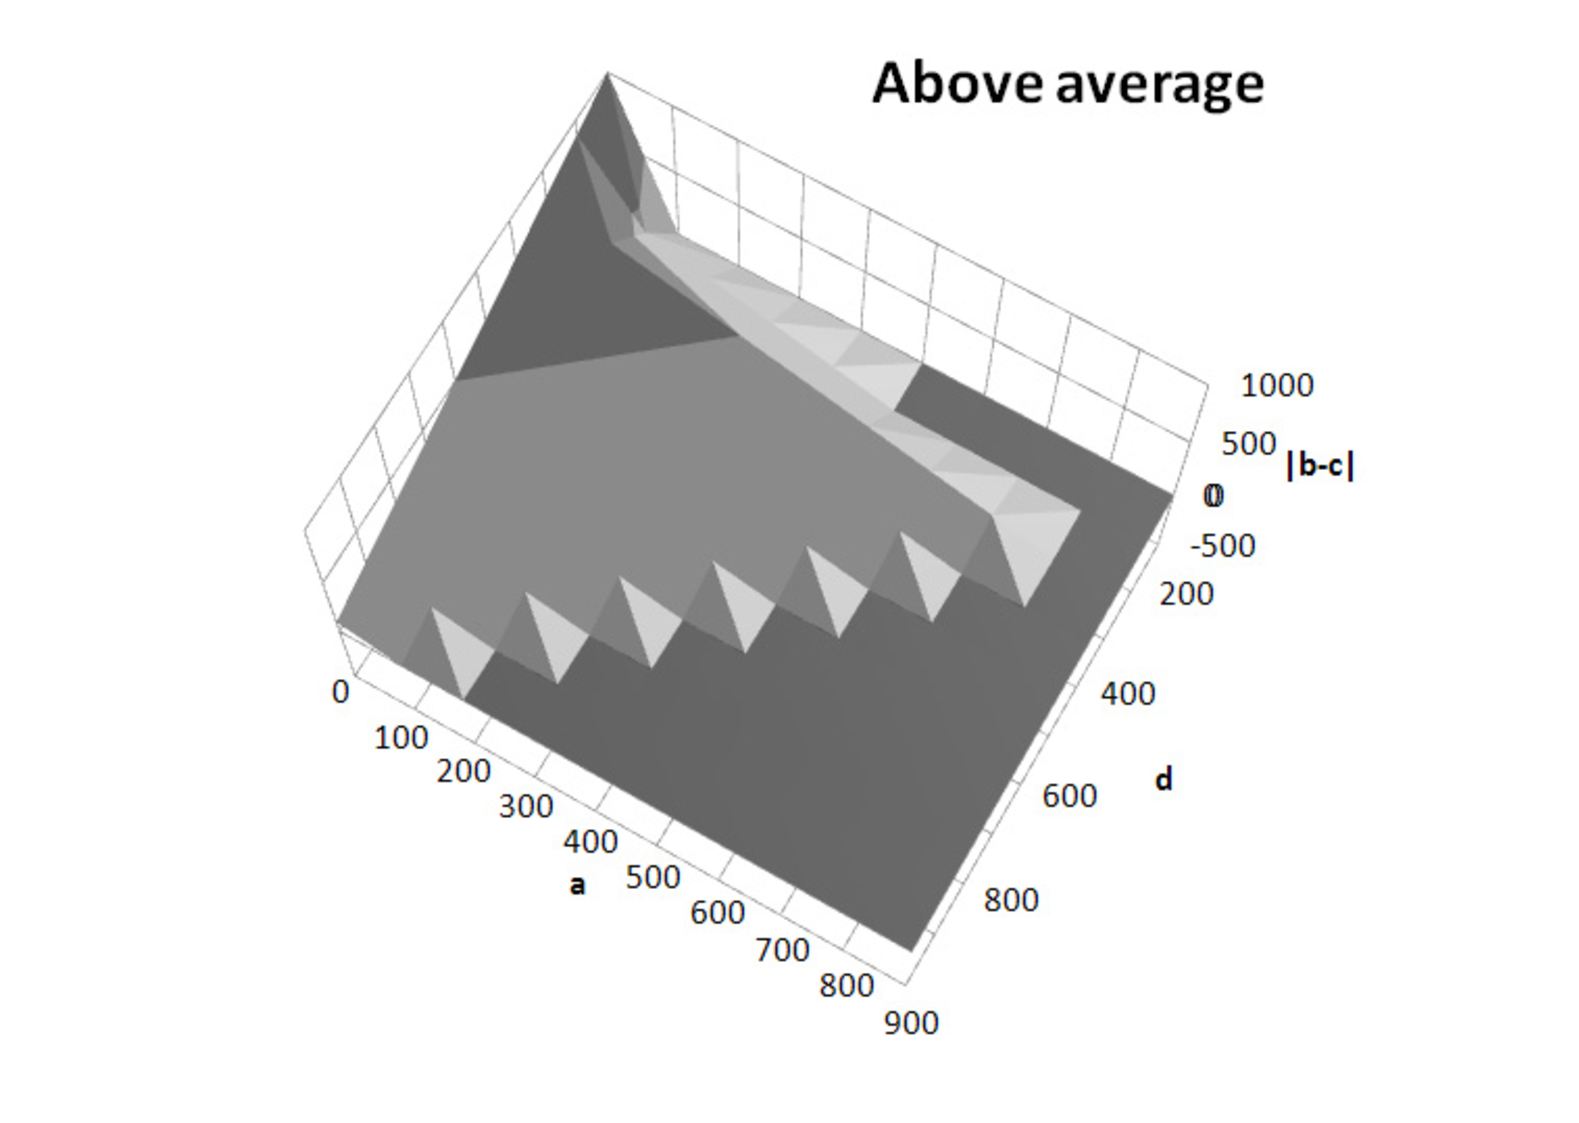
\includegraphics[width=70mm]{AA.eps}
%\mbox{\resizebox{125mm}{!}{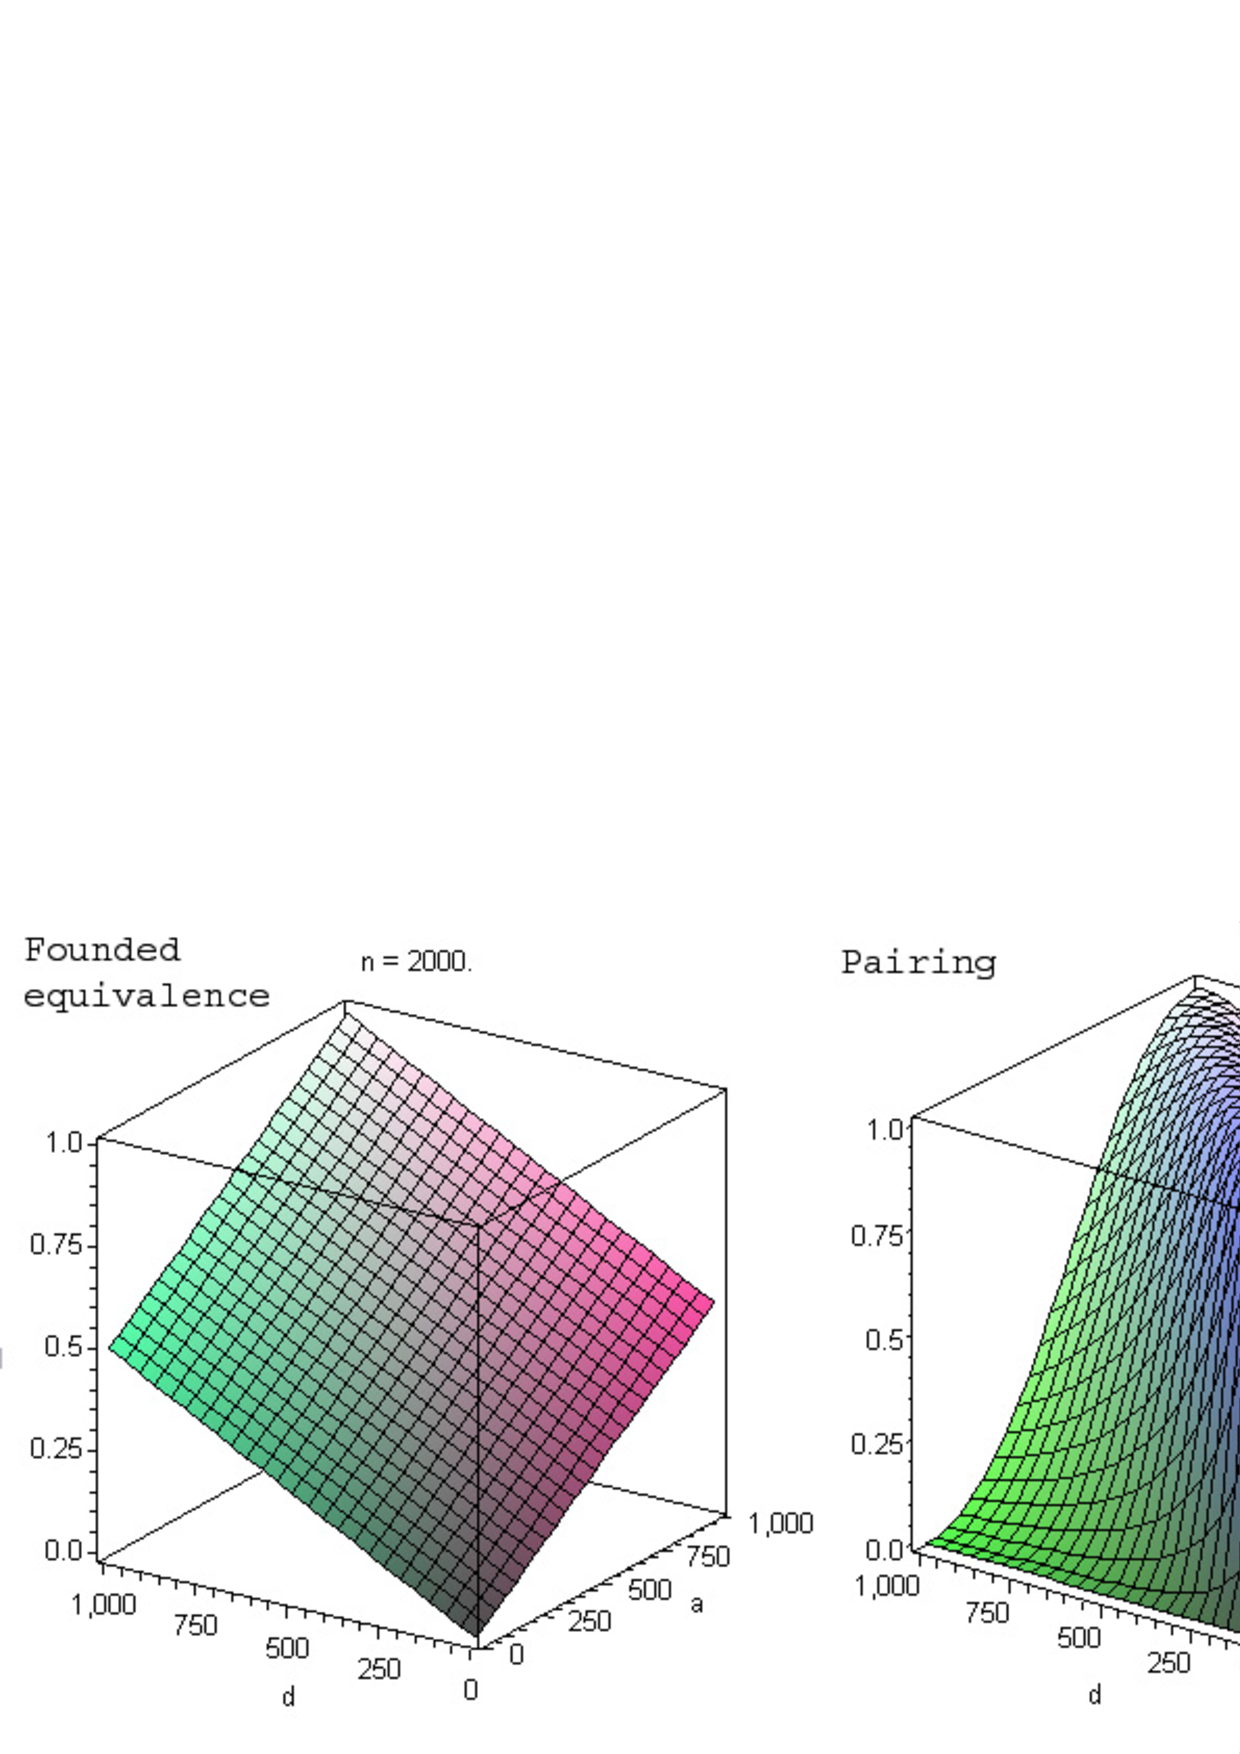
\includegraphics{FE-Pairing.png}}}
\caption{Tables of minimal $|b-c|$ for Above average dependence quantifier}
\label{fig:AA}
\end{figure}

We also examined the graph of \emph{above average dependence} and made comparison with the \emph{simple deviation} graph. The latter can be naturally interpreted as a plane that rises inversely with the $ad$ axis. The slope of the plane is determined by the $\delta$ parameter. The \emph{above average dependence} graph is shown in figure \ref{fig:AA}, with $n=1000$ and $p=0.2$. Shapes of the graphs are similar except for region with high $a$ and low $d$. In this region the \emph{above average dependence} the quantifier is not valid at all. This can be explained by the fact, that with high values of $a$ (with respect to $n$, size of the table) and low values of $d$, the two fractions from the quantifier's condition $ \frac{a}{a+b} \geq (1+p) \frac{a+c}{a+b+c+d} $ tend to have the same value, therefore it is hard for $b$ and $c$ to fulfill the inequality. 

Again, the graphical analysis tells us more about the quantifier's usage. Although the \emph{above average dependence} proved to be usable in many applications, the discussion in previous paragraph showed that in special cases (for very low $d$ and high $a$) the quantifier does not behave as expected. With common sense, association with high $a$ with respect to $n$ should be considered as good. The \emph{above average dependence} does not give this result. 